% !TeX spellcheck = ru_RU-Russian
\documentclass[a4paper, fontsize=14pt]{article} 
\usepackage{course_work}
\addbibresource{report.bib}
\bibliography{report.bib}
%\usepackage{graphs/gnuplot-lua-tikz}
%\setcounter{page}{4} %в зависимости от того, какой по счёту страницей должно
%быть оглавление!
%\usepackage{pstricks}
\newcommand{\divop}{\operatorname{div}}
\newcommand{\gradop}{\operatorname{grad}}
\begin{document} 
	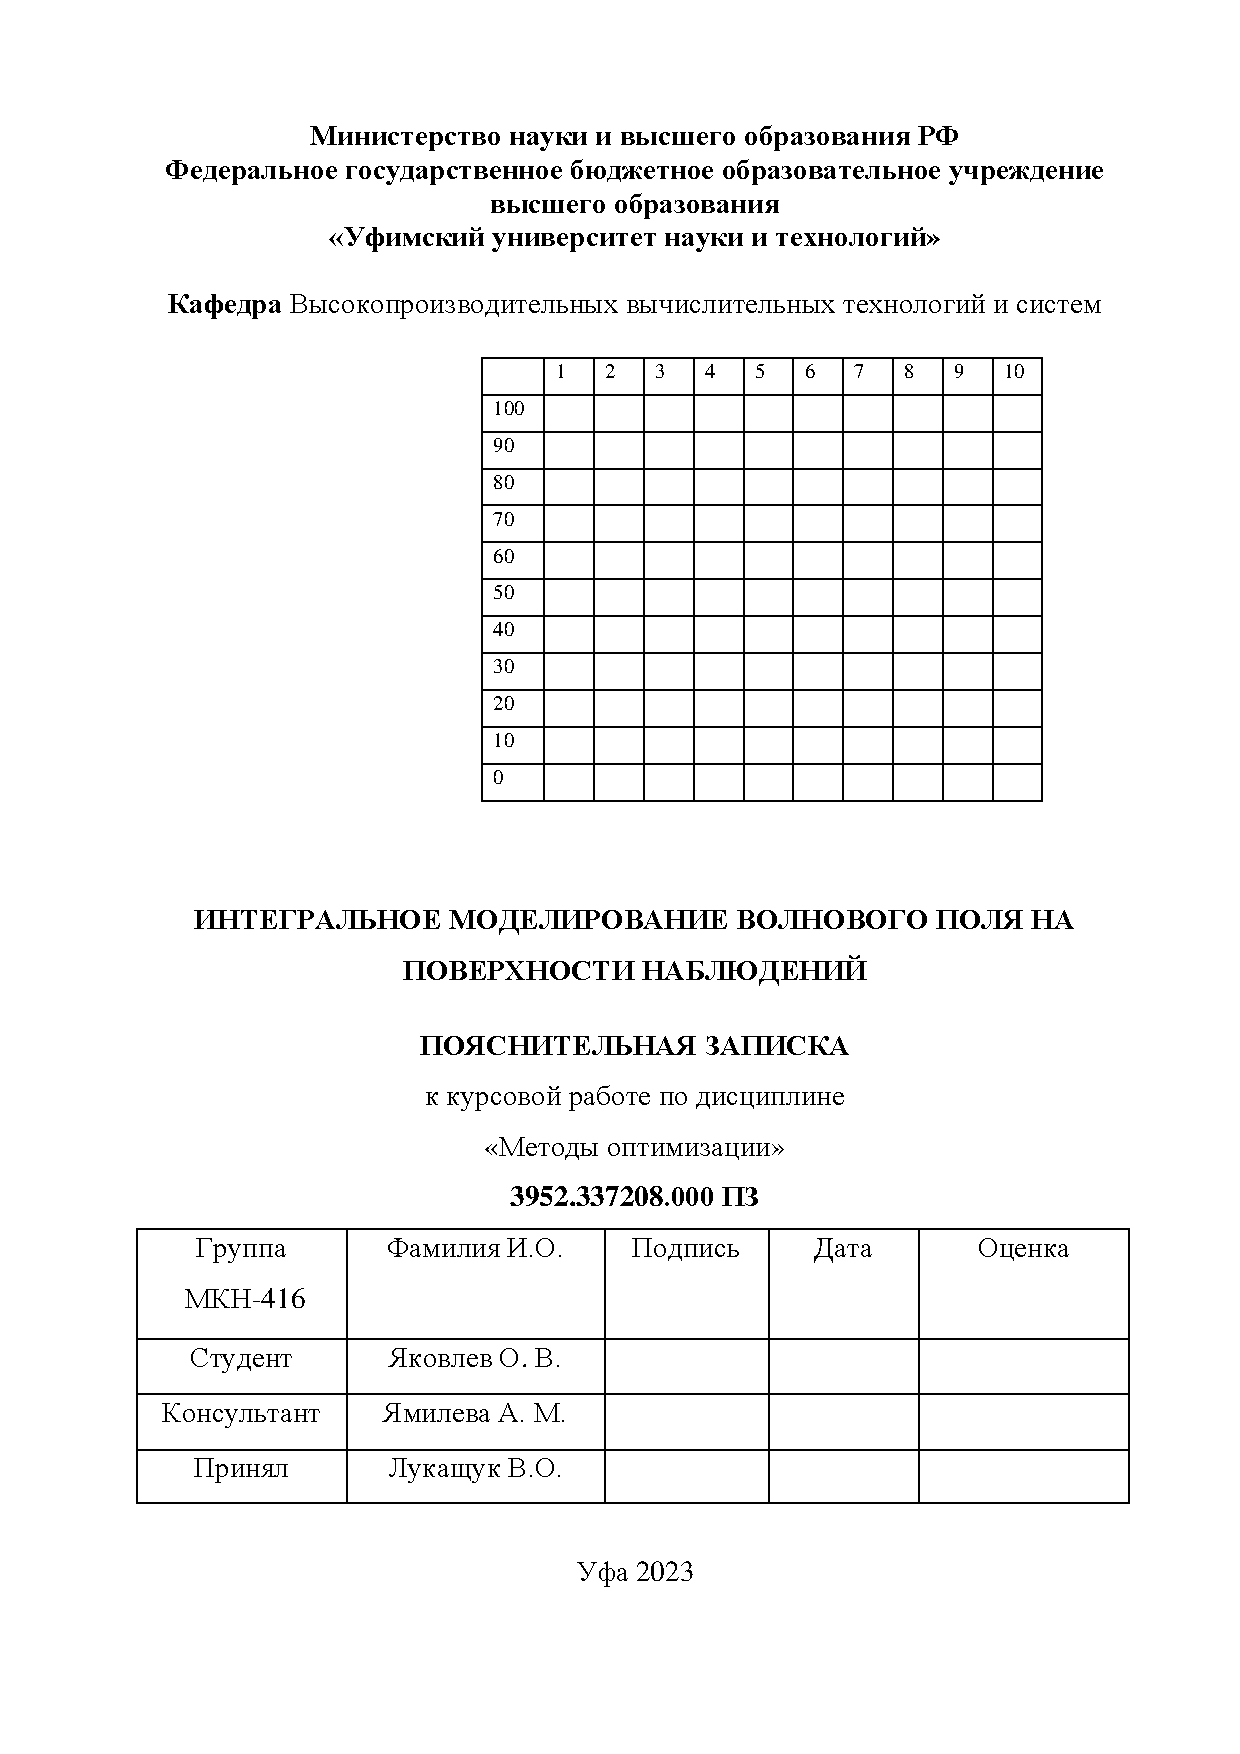
\includepdf[pages=1-3]{cover.pdf} \newpage \tableofcontents
	\newpage 
	\section*{Введение} 
	\addcontentsline{toc}{section}{Введение}
	
	
	\newpage 
	\section{Постановка задачи} 
	\begin{figure}[h]
		
		\centering
		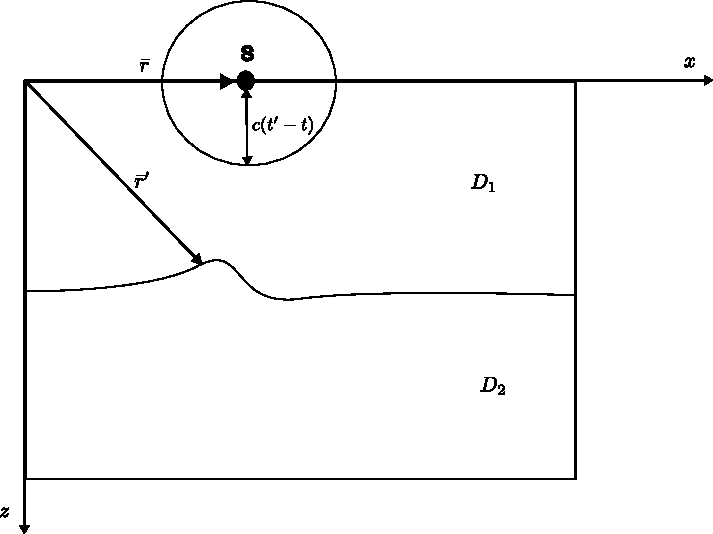
\includegraphics{migration_fig.pdf}
		
		\caption{Модель среды}
		\label{fig:mig}
	\end{figure}
	Рассмотрим задачу нахождения значения скалярного волнового поля на поверхности
	наблюдения.
	Допустим задана поверхность, ограничивающая некоторую область пространства
	$D=[0,X]\times [0,Y]\times [0,Z]$, изображённую на рисунке \ref{fig:mig}.
	Область пространства $D$ разделена на слои $D_1$ и $D_2$, с постоянной
	скоростью звука $c_1$ и $c_2$ соответственно.
	На границе находятся точечные источники колебаний $S$, которые возбуждают
	акустическую волну.
	
	Необходимо по данным характеристикам источников найти значение отражённого волнового поля
	на поверхности наблюдения $z=0$.
	
	\section{Волновое уравнение}
	Конечно, решение данной задачи можно получить при помощи решения
	дифференциального волнового уравнения \ref{eq:wav}. 
	\begin{equation}
		\frac{\partial^2 P}{\partial x^2} + \frac{\partial^2 P}{\partial y^2} +
		\frac{\partial^2 P}{\partial z^2} - \frac{1}{c^2} \frac{\partial^2 P}{\partial
			t^2} = -F(x,y,z,t)   
		\label{eq:wav}	
	\end{equation}
	Однако, для волнового уравнения с произвольной правой частью $F(x,y,z,t)$ можно
	записать формулу представления решения 
	в аналитическом виде при помощи функции Грина, введя вектор $\bar{r} = (x,y,z)$.
	\begin{equation}
		P(\bar{r}',t')=\iiint\limits_{D_1} \int\limits_{-\infty}^{+\infty}
		F(\bar{r},t) G(\bar{r}',t'|\bar{r},t)\,dt\,dv
	\end{equation}
	%%%%%%%%%%%%%%%%%%%%%%%%%%%%%%%%%%%
	\section{Функция Грина} 
	
	Рассмотрим мгновенный точечный источник колебаний в трёхмерном пространстве.
	Тогда правая часть уравнения \ref{eq:wav} будет иметь вид \cite{zhdanov1988}
	\begin{equation}
		F(x,y,z,t) = \delta(t-t')\delta(x-x')\delta(y-y')\delta(z-z')
		\label{eq:ptsrc}
	\end{equation}
	Где $\delta(x)$ -- это дельта-функция Дирака.
	\begin{equation}
		\delta(x)=\begin{cases}
			\infty,&x=0\\
			0,&x\neq 0
		\end{cases}
		\label{eq:deltadef}
	\end{equation}	
	Решением уравнения \ref{eq:wav} с правой частью \ref{eq:ptsrc} является функция
	Грина для волнового уравнения в трёхмерном пространстве.
	
	Пусть источник колебаний находится в начале координат и время импульса $t' = 0$. 
	
	Так как правая часть уравнения равна 0 везде, кроме точки $O(0,0,0)$, поэтому 
	$G$ удовлетворяет уравнению \ref{eq:uwav} всюду, кроме начала координат
	\begin{equation}
		\frac{\partial^2 G}{\partial x^2} + \frac{\partial^2 G}{\partial y^2} +
		\frac{\partial^2 G}{\partial z^2} - \frac{1}{c^2} \frac{\partial^2 G}{\partial
			t^2} = 0.
		\label{eq:uwav}
	\end{equation}
	Учитывая сферическую симметрию функции Грина, перейдём в уравнении \ref{eq:uwav} к сферической системе координат
	\begin{equation}
		\frac{1}{r^2}\frac{\partial}{\partial r}\left( r^2 \frac{\partial G}{\partial r} \right)- \frac{1}{c^2} \frac{\partial^2 G}{\partial
			t^2} = 0.
		\label{eq:uswav}
	\end{equation}
	Воспользовавшись равенством $\frac{1}{r}\frac{\partial}{\partial r}\left(r^2\frac{\partial G}{\partial r}\right) = \frac{\partial^2}{\partial r^2}\left(rG\right)$ преобразуем уравнение \ref{eq:uswav}:
	\begin{equation}
		\frac{\partial^2}{\partial r^2}\left( r  G\right)- \frac{1}{c^2} \frac{\partial^2 }{\partial
			t^2}\left(r G\right) = 0.
		\label{eq:uswav2}
	\end{equation}
	Таким образом мы смогли свести уравнение к одномерному волновому уравнению относительно $F(r,t) = rG$. При помощи замены переменных $\xi = t - \frac{r}{c}$, $\eta = t+\frac{r}{c}$ к простому виду:
	\begin{equation}
		\frac{\partial^2}{\partial \xi \partial \eta} F = 0	
		\label{eq:canonwav}
	\end{equation}
	Интегрируя уравнение \ref{eq:canonwav}, выразим значение функции Грина из решения дифференциального уравнения:
	\begin{equation}
		G(x,y,z,t) = \frac{1}{r}f\left(t-\frac{r}{c}\right) + \frac{1}{r} g\left(t+\frac{r}{c}\right),
		\label{eq:canonsol}
	\end{equation}
где $r = \sqrt{x^2+y^2+z^2}$.

Первое слагаемое выражения \ref{eq:canonsol}  описывает сферическую волну, распространяющуюся от начала координат в бесконечность., а второе слагаемое -- сферическую волну из бесконечности к началу координат. Поскольку, по условиям задачи, источником колебания является единственный источник, то функцию $g$ примем равной нулю.  Чтобы найти функцию  $f$  подставим решение \ref{eq:canonsol} в уравнение \ref{eq:wav}. 
\begin{equation}
	\Delta \left[ \frac{1}{r}f\left(t-\frac{r}{c}\right) \right] - \frac{1}{c^2} \frac{\partial^2 }{\partial
		t^2}\left[ \frac{1}{r}f\left(t-\frac{r}{c}\right) \right]  = - \delta(t)\delta(x)\delta(y)\delta(z)
		\label{eq:fwav}
\end{equation}
Используя равенство $\Delta\left(\frac{1}{r}\right) = -4\pi \delta(x)\delta(y)\delta(z)$, можно привести уравнение \ref{eq:fwav}
к виду 
\begin{equation}
	-4\pi f(t) \delta(x) \delta(y) \delta(z)  = \delta(x) \delta(y) \delta(z) \delta(t),
\label{eq:fdel}	
\end{equation}
откуда можно выразить значение функции Грина:
\begin{equation}
	G(x,y,z,t) = -\frac{1}{4\pi r} \delta \left(t - \frac{r}{c}\right),
\label{eq:green3d0}	
\end{equation}  
где $r = \sqrt{x^2+y^2+z^2}$.

При выводе формулы \ref{eq:green3d0} использовалось предположение,  что источник находится в начале координат  и посылает импульс в момент времени $t' = 0$. При переходе к произвольному положению источника 
формула для функции Грина имеет вид
\begin{equation}
	G(\bar{r}',t'|\bar{r},t)= \frac{1}{4\pi|\bar{r}'-\bar{r}|}
	\delta\left(t'-t-\frac{|\bar{r}'-\bar{r}|}{c}\right)
\label{eq:green3d}
\end{equation}

	Такая функция Грина называется запаздывающей функцией Грина, так как эффект,
	наблюдаемый в точке $\bar{r}'$ в более поздний момент времени $t'$ вызывается
	возмущением,
	которое произошло в точке $\bar{r}$ в более ранний момент времени $t$.

	%TODO: \textbf{TODO} написать вывод функции Грина
	
% Связь излучаемого и отраженного волнового поля через коэффициент отражения

	\section{Формула Кирхгофа}
	Для вычисления значения отражённого волнового поля на поверхности наблюдения необходимо 
	рассмотреть как связано значение поля на отражающей границе и значения поля в других точках области, которую ограничивает эта поверхность.   
	
	Рассмотрим  некоторую ограниченную область пространства $D$, в пределах которой задано скалярное волновое поле, удовлетворяющее уравнению \ref{eq:uwav2}. Положим, что граница $S$ области $D$ является кусочно-гладкой.
	
	\begin{equation}
		\diff[2]{P}{x}  + \diff[2]{P}{y} +
		\diff[2]{P}{z}  - \frac{1}{c^2} \frac{\partial^2 P}{\partial
			t^2} = 0.
		\label{eq:uwav2}
	\end{equation}
	
	Так как область $D$ ограничена и имеет кусочно-гладкую границу, тогда по
	теореме Остроградского-Гаусса справедливо соотношение
	\begin{equation}
		\iiint\limits_D \divop F \, dv = \iint\limits_S F \cdot n \, ds 
		\label{eq:vgauss}
	\end{equation}
	Для любых гладких функций $u$ и $v$ справедливо соотношение 
	\begin{equation}
		\divop (u \gradop v) = u\Delta v + \gradop u \cdot \gradop v.
		\label{eq:divgrad1}
	\end{equation}
	Симметрично можно записать:
	\begin{equation}
		\divop (v \gradop u) = v\Delta u + \gradop v \cdot \gradop u.
		\label{eq:divgrad2}
	\end{equation}
	Путём вычитания из уравнения \ref{eq:divgrad1} уравнения \ref{eq:divgrad2} получим 
	\begin{equation}
		\divop (u \gradop v - v \gradop u)  = u\Delta v - v \Delta u
		\label{eq:divgraddiff}
	\end{equation}
	Положим 
	\begin{eqnarray}
		u(x,y,z,t) =& P(x,y,z,t),\label{eq:subsu}\\
		v(x,y,z,t) = &G(x,y,z,t)\label{eq:subsv},
	\end{eqnarray}	
	тогда 
	% TODO  Ввести вектора r и r'
\begin{eqnarray}
	\Delta u =& \frac{1}{c^2} \diff[]{P}{t},\label{eq:subsdu}\\
	\Delta v = &\delta (r' - r) \delta(t' - t) + \frac{1}{c^2} \diff [2]{G(r' -r,t'-t)}{t}.\label{eq:subsdv}
\end{eqnarray}
	Проинтегрируем уравнение \ref{eq:divgraddiff} по времени
	\begin{equation}
		\divop \int\limits_{-\infty}^{+\infty} [P \gradop G - G \gradop P ]\, dt=  P\delta(r-r') +\frac{1}{c^2}\int\limits_{-\infty}^{+\infty}\left[P\diff[2]{G}{t} - G \diff[2]{P}{t}\right]\,dt.
		\label{eq:ugauss}
	\end{equation}
	Интегрированием по частям можно показать, что 
	$$
	\int\limits_{-\infty}^{+\infty}\left[P\diff[2]{G}{t} - G \diff[2]{P}{t}\right]\,dt = 0.
	$$
	Введём обозначение 
	$$
		F(x,y,z,t') = \int\limits_{-\infty}^{+\infty} [P \gradop G - G \gradop P ]\, dt
	$$
	Тогда из уравнений \ref{eq:ugauss} и \ref{eq:vgauss} следует
	\begin{equation}
		\iiint\limits_D P\delta(r-r') \, dv = \iint\limits_S F \cdot n \, ds 
	\end{equation}
Таким образом, 
	\begin{equation}
		P(r',t') = \iint\limits_{\partial D} \int\limits_{-\infty}^{+\infty} 
	[G(r',t'|r,t)\partial_n P(r,t) 
	- P(r,t)\partial_n G(r',t'|r,t)] \,dt\,ds
	\label{eq:kir}
	\end{equation}
	
	
	Это соотношение носит название интегральной формулы Кирхгофа.
	Интегральная
	формула Кирхгофа показывает, как можно восстановить волновое поле внутри области,
	ограниченной некоторой поверхностью, по значениям этого поля (и его нормальной
	производной) на границе области.
	% 
	%TODO:	\textbf{TODO} написать вывод интеграла кирхгофа
	
	
	
	
	
	\clearpage
	
	
	\section*{Заключение} \addcontentsline{toc}{section}{Заключение}
	
	\newpage
	
	\addcontentsline{toc}{section}{Список литературы}
	
	\printbibliography
	
	\newpage
	
	\includepdf[pages=11]{cover.pdf}
	
\end{document}


